\documentclass[a4paper, 11pt]{article}

\usepackage{fullpage}

\usepackage[english,russian]{babel}
\usepackage[utf8]{inputenc}
\usepackage{amsmath, amsfonts, amssymb, amsthm}
\usepackage{mathtools}
\usepackage{bm}

\usepackage{hyperref}
\usepackage{booktabs}
\usepackage{graphicx}
\usepackage{subcaption}

\usepackage[linesnumbered,ruled,vlined]{algorithm2e}
\SetKwInput{KwInput}{input}
\SetAlFnt{\small}

\usepackage{float}

\newtheorem{definition}{Определение}
\newtheorem{theorem}{Теорема}
\newtheorem{lemma}{Лемма}

\begin{document}

\begin{titlepage}
	\newpage
	
	\begin{center}
		%	Московский Государственный Университет им. М. В. Ломоносова \\
	\end{center}
	
	\vspace{8em}
	
	\begin{center}
		%\Large Кафедра Вычислительных Технологий и Моделирования \\ 
	\end{center}
	
	\vspace{2em}
	
	\begin{center}
		\textsc{\textbf{Численное решение задач течения подземных вод}}
	\end{center}
	
	\vspace{6em}
	
	
	
	\newbox{\lbox}
	\savebox{\lbox}{\hbox{}}
	\newlength{\maxl}
	\setlength{\maxl}{\wd\lbox}
	\hfill\parbox{11cm}{
		%\hspace*{5cm}\hspace*{-5cm}Студент:\hfill\hbox {Иванов И. И.\hfill}\\
		%\hspace*{5cm}\hspace*{-5cm}Преподаватель:\hfill\hbox {Ануприенко Д. В.\hfill}\\
		%	\\
		%\hspace*{5cm}\hspace*{-5cm}Группа:\hfill\hbox {403}\\
	}
	
	
	\vspace{\fill}
	
	\begin{center}
		Москва \\ 2025
	\end{center}
	
\end{titlepage}

\setcounter{MaxMatrixCols}{20}

\section{Метод конечных разностей для одномерного уравнения Пуассона}

\subsection{Постановка задачи}

Многие стационарные, то есть установившиеся, не меняющиеся во времени процессы (распространение тепла, распределение электрических зарядов, течение подземных вод) в одномерных объектах (телах, у которых одно из измерений существенно больше остальных, например: стержнях, тонких колонках из пористого материала и др.) описываются следующими уравнениями:

\begin{equation}\label{eq:2eq_1d}
	\begin{cases}
		\frac{\partial q}{\partial x} = f(x),\\
		q(x) = -\frac{\partial u}{\partial x},
	\end{cases}
\end{equation}

где $u$ -- основная неизвестная (температура, напор подземных вод, электрический потенциал, концентрации примеси в жидкости и др.), $q$ --  поток (тепла, массы, заряда и т.д.), а $f$ -- функция источников. Первое уравнение в \eqref{eq:2eq_1d} описывает закон сохранения (тепла, массы, заряда) в дифференциальной форме, а второе уравнение говорит о том, что движение происходит от области с большей температурой (напором, потенциалом) в область с меньшей (в некоторых разделах физики эти законы имеют имена -- закон Фурье, закон Фика, закон Дарси и др.).

Соединив два уравнения в \eqref{eq:2eq_1d}, можно получить уравнение Пуассона:

\begin{equation}
	-\frac{\partial^2 u}{\partial x^2} = f(x).
\end{equation}

Очевидно, что у этого уравнения бесконечно много решений. Чтобы получить практически значимое единственное решение, нужно рассмотреть уравнение в конкретной области (далее для простоты -- на единичном отрезке) и задать некоторую информацию на границах:

\begin{equation}\label{eq:poisson_bvp_dir_1d}
	\begin{cases}
		-\frac{\partial^2 u}{\partial x^2} = f(x),~~x\in\Omega = (0,L),\\
		u(0) = a, u(L) = b
	\end{cases}
\end{equation}

Система \eqref{eq:poisson_bvp_dir_1d} называется \textit{краевой задачей} для уравнения Пуассона, заданные на границах отрезка значения искомой функции $u$ -- \textit{граничными условиями}. Граничные условия такого типа называются условиями Дирихле. В случае, когда вместо исходной функции задан поток $q$, граничное условие называется условием Неймана.

\subsection{Метод конечных разностей}
Краевая задача \eqref{eq:poisson_bvp_dir_1d}, конечно, может быть решена аналитически. Однако при переходе к многомерным задачам, областям $\Omega$ сложной формы, единственным вариантом в большинстве случаев является численное решение. Рассмотрим подходы к нему на примере простой одномерной задачи.
\begin{figure}[h] \centering
	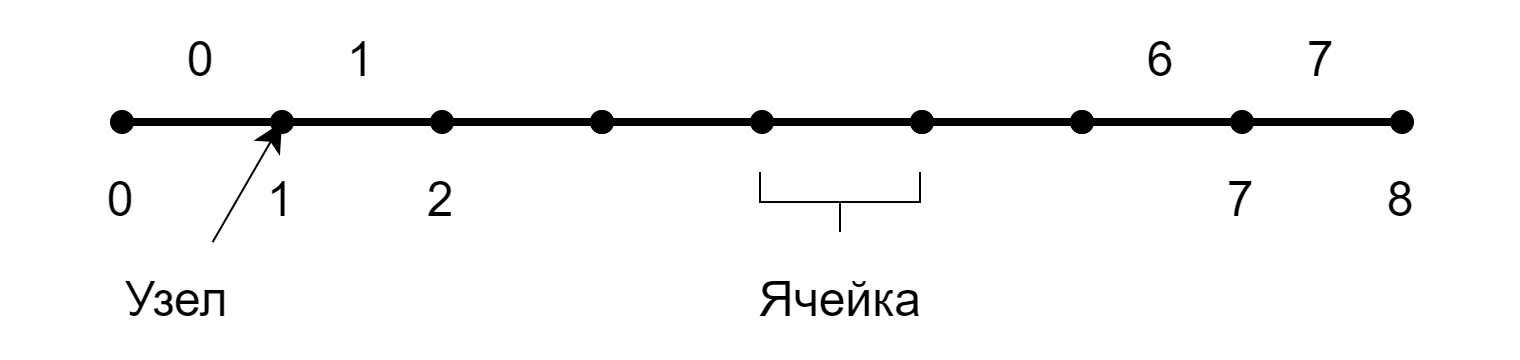
\includegraphics[width=\textwidth]{mesh1d}
	\caption{Одномерная сетка с номерами узлов снизу и номерами ячеек сверху\label{pic:mesh1d}}
\end{figure}

Первым делом выполняется разбиение расчетной области (в нашем случае -- отрезка) на маленькие отрезки. Это разбиение называется сеткой (см. рис. \ref{pic:mesh1d}). Точки разбиения называются узлами, а получающиеся отрезки -- ячейками. Вводя сетку с $N$ ячейками, мы имеем $N+1$ узлов и шаг сетки, то есть размер ячейки, равный $\Delta x = L/N$. Формально говоря, узлы имеют координаты $x_i = i\Delta x,~~i = 0, \dots, N$. Ячейка с номером $i$ представляет собой отрезок $[x_i, x_{i+1}]$.

Решением краевой задачи \eqref{eq:poisson_bvp_dir_1d} в классическом смысле является некоторая функция $u \in C^2(0,L) \cap C[0;1]$ и т.д. и т.п. В численном же решении мы будем искать набор значений в узлах:
\begin{equation}
	y_i \approx u(x_i),~~~i = 0, \dots, N.
\end{equation}

Поскольку значения в граничных узлах определяются граничными условиями, фактически задача сводится к поиску $y_1, ..., y_{N-1}$. 

Идея метода конечных разностей состоит в замене производных в уравнении на некоторые конечные разности. Так, например, можно использовать выражения
\begin{equation}\label{eq:differences_1}
	\begin{split}
		y_{x,i} = \frac{y_{i+1} - y_i}{\Delta x} = u'(x_i) + \mathcal{O}(\Delta x),\\
		y_{\overline{x},i} = \frac{y_i - y_{i-1}}{\Delta x} = u'(x_i) + \mathcal{O}(\Delta x),
	\end{split}
\end{equation}
называемые разностными производными вперед и назад. Оценки на погрешность аппроксимации справедливы для достаточно гладких функций.

Разностная аппроксимация второй производной имеет вид
\begin{equation}\label{eq:differences_2}
	\begin{split}
		y_{x\overline{x},i} \equiv y_{\overline{x}x,i} = \frac{y_{i+1} - 2y_i + y_{i-1}}{\Delta x^2} = u''(x_i) + \mathcal{O}(\Delta x^2).
	\end{split}
\end{equation}

Для определения значений $y_i$ составляется система линейных алгебраических уравнений. В каждом внутреннем узле исходное уравнение заменяется на разностную аппроксимацию:
\begin{equation}
	\begin{cases}
		-\frac{y_{2} - 2y_1 + a}{\Delta x^2} = f(x_1),\\
		-\frac{y_{3} - 2y_2 + y_1}{\Delta x^2} = f(x_2),\\
		\dots\\
		-\frac{y_{i+1} - 2y_i + y_{i-1}}{\Delta x^2} = f(x_i),
		\dots\\
		-\frac{b - 2y_{N-1} + y_{N-2}}{\Delta x^2} = f(x_{N-1})\\
	\end{cases}
\end{equation}

Если умножить все уравнения на $\Delta x ^2$, в матричном виде система принимает следующий вид:
\begin{equation}\label{eq:matrix_fd_1d}
	\begin{bmatrix}
		2  & -1 &   &       \\
		-1 &  2 & -1 \\
		   & -1 &  2 \\
		   &    &   & \ddots \\
		   &    &   &       &  & -1\\
		   &    &   &       & -1 & 2
		
	\end{bmatrix}
	\begin{bmatrix}
		y_1 \\ y_2 \\ y_3 \\ \vdots \\y_{N-2} \\ y_{N-1}
	\end{bmatrix}
	=
	\Delta x^2 
	\begin{bmatrix}
		f(x_1) + a/\Delta x^2 \\
		f(x_2)\\
		f(x_3)\\
		\vdots\\
		f(x_{N-2})\\
		f(x_{N-1}) + b/\Delta x^2 
	\end{bmatrix}
\end{equation}

Матрица системы является симметричной, знакоопределенной и разреженной (число ненулевых элементов порядка размера матрицы). Это типично для матриц, возникающих при дискретизации уравнений в частных производных. Обычно для решения таких линейных систем применяются специальные методы, учитывающие свойства матрицы. В данном случае для трехдиагональной матрицы можно применить метод прогонки, имеющий идеальную сложность $\mathcal{O}(N)$.

\subsection{Метод конечных объемов}
 Метод конечных объемов (англ. finite volume method), также известный как метод контрольного объема, интегро-интерполяционный метод и метод баланса– метод дискретизации уравнений в частных производных, хорошо подходящий для уравнений, включающих
законы сохранения (подобно уравнениям \eqref{eq:2eq_1d}). Идея состоит в записи закона сохранения
в интегральной форме на каждой ячейке (так называемом конечном объеме). Для этого
первое уравнение в \eqref{eq:2eq_1d} интегрируется по ячейке:

\begin{equation}
	\int_{x_i}^{x_{i+1}} \frac{\partial q}{\partial x}dx = \int_{x_i}^{x_{i+1}} f(x)dx,
\end{equation}

\begin{equation}
	q_{i+1} - q_i = \int_{x_i}^{x_{i+1}} f(x)dx,
\end{equation}

 Иначе говоря, разность потоков через границы ячейки равна интегральному значению
источника в ячейке. Теперь необходимо как-то выразить потоки и аппроксимировать интеграл в правой части. В МКО это делается достаточно просто. Важное отличие от МКР заключается в том, что дискретные неизвестные относятся к ячейкам, а не к узлам! То есть,
вместо поиска неизвестных $y_1, \dots, y_{N-1}$, соответствующих значениям во внутренних узлах,
ищутся значения $y_0, \dots, y_{N-1}$, соответствующие значениям в центрах ячеек:

\begin{equation}
	y_i \approx u(x_{i+1/2}).
\end{equation}

Далее потоки в узлах выражаются конечными разностями с использованием в двух
соседних ячейках, разграничивающихся узлом:

\begin{equation}
	-\frac{y_{i+1} - y_i}{\Delta x} + \frac{y_i - y_{i-1}}{\Delta x} = \int_{x_i}^{x_{i+1}} f(x)dx,
\end{equation}

 Осталось аппроксимировать интеграл в правой части. Сделаем это с использованием
значения источника в центре ячейки:

\begin{equation}
	-\frac{y_{i+1} - y_i}{\Delta x} + \frac{y_i - y_{i-1}}{\Delta x} = f(x_{i+1/2})\Delta x.
\end{equation}

Такие уравнения справедливы для внутренних ячеек. Для граничных ячеек с номерами $0$ и $N-1$ несколько отличается аппроксимация потока. Конечная разность в этих случаях берется между
значением в центре граничной ячейки и значением на границе, которые разделяет расстояние $\Delta x / 2$, а не $\Delta x$:

\begin{equation}
	-\frac{y_1 - y_0}{\Delta x} + \frac{y_0 - a}{\Delta x / 2} = f(x_{1/2})\Delta x,
\end{equation}
\begin{equation}
	-\frac{b - y_{N-1}}{\Delta x / 2} + \frac{y_{N-1} - y_{N-2}}{\Delta x} = f(x_{N-1/2})\Delta x.
\end{equation}

Матричное представление системы следующее (если, как и в МКР, умножить уравнения на $\Delta x$):
\begin{equation}\label{eq:matrix_1d_fv}
	\begin{bmatrix}
		3  & -1 &   &       \\
		-1 &  2 & -1 \\
		& -1 &  2 \\
		&    &   & \ddots \\
		&    &   &       &  2 & -1\\
		&    &   &       & -1 & 3
		
	\end{bmatrix}
	\begin{bmatrix}
		y_0 \\ y_1 \\ y_2 \\ \vdots \\y_{N-2} \\ y_{N-1}
	\end{bmatrix}
	=
	\Delta x^2 
	\begin{bmatrix}
		f(x_{1/2}) + 2a/\Delta x^2 \\
		f(x_{1+1/2})\\
		f(x_{2+1/2})\\
		\vdots\\
		f(x_{N-3/2})\\
		f(x_{N-1/2}) + 2b/\Delta x^2 
	\end{bmatrix}
\end{equation}

Эта система очень похожа на систему \eqref{eq:matrix_fd_1d}, полученную методом конечных разностей. Решение системы выполняется аналогично. На одномерных задачах 
разница решений практически незаметна, однако на более сложных задачах автоматическое выполнение закона сохранения массы в МКО позволяет получать физически более
корректные решения.

\section{Стационарное уравнение фильтрации в неоднородной одномерной области}
\subsection{Постановка задачи}
Уравнения модели похожи на приведенные в начале уравнения \eqref{eq:2eq_1d}. Уточним их со специфической для подземных вод терминологией и учетом неоднородности области. Уравнения имеют вид

\begin{equation}\label{eq:2eq_1d_het}
	\begin{cases}
		\frac{\partial q}{\partial x} = f(x),\\
		q(x) = -K(x)\frac{\partial h}{\partial x},
	\end{cases}
\end{equation}

куда входят следующие величины (далее $L$ -- единицы длины, $T$ -- единицы времени):
\begin{itemize}
	\item $h$ -- напор воды (англ. water head), основная неизвестная, [$L$];
	\item $q$ -- поток воды (англ. flux), [$LT^{-1}$];
	\item $K(x)$ -- меняющийся по пространству коэффициент фильтрации (как правило -- кусочно-постоянный на ячейках), [$LT^{-1}$]; 
	\item $f(x)$ -- источники и стоки, как правило, связанные с работой закачивающих или откачивающих скважин и подобных объектов, [$T^{-1}$].
\end{itemize}

Эти уравнения описывают течение подземных вод в так называемых напорных условиях, когда поры среды заполнены водой до конца. Коэффициент фильтрации определяет способность среды пропускать воду.

\subsection{Метод конечных объемов}
Поскольку первое уравнение в системах \eqref{eq:2eq_1d} и \eqref{eq:2eq_1d_het} одинаково, так как описывает закон сохранения массы, отличие в построении схемы МКО заключается в выражении для потока, которое теперь должно учитывать неоднородность среды. 

Построим выражение для потока через узел $i$, разграничивающий ячейки с номерами $i$ и $i-1$, имеющие коэффициенты фильтрации $K_{i-1}$ и $K_i$. Для этого введем вспомогательное значение напора в разграничивающем узле -- $h_*$, и запишем с помощью него потоки в обеих ячейках:

\begin{equation}
	q_{left} = -K_{i-1}\frac{h_* - h_{i-1}}{\Delta x/2},
\end{equation}
\begin{equation}
	q_{right} = -K_i\frac{h_{i} - h_*}{\Delta x/2}.
\end{equation}

Если приравнять эти потоки и выразить $h_*$, то выражение для потока через узел $i$ получится следующим:
\begin{equation}
	q_i = -\frac{2K_i K_{i-1}}{K_{i-1} + K_i}\frac{h_i - h_{i-1}}{\Delta x},
\end{equation}
что является, подобно случаю уравнения Пуассона, конечной разностью с коэффициентом фильтрации, вычисленным по формуле среднего гармонического. 

Для потоков на границе среднее гармоническое не используется, берется значение коэффициента фильтрации из ячейки.

Итоговая система уравнений является, как и ранее, линейной системой вида 
\begin{equation}\label{eq:Ahp}
	Ah = p,
\end{equation}

где $A$ -- трехдиагональная матрица, $h$ -- вектор значений напора в ячейках сетки, а $p$ -- вектор правой части, содержащий вклад от источников/стоков и граничных условий. 


\section{Нестационарное уравнение фильтрации в неоднородной одномерной области}
\subsection{Постановка задачи}
Эта задача отличается введением времени, то есть решение (напор) зависит не только от пространственной координаты $x$, но и от времени $t$, то есть $h = h(x,t)$. Задача ставится следующим образом:

\begin{equation}\label{eq:ivp_conf_1d}
	\begin{cases}
		s_{stor}(x)\frac{\partial h}{\partial t} - \frac{\partial}{\partial x}\left(K(x)\frac{\partial h}{\partial x}\right) = f(x), ~~~~ x \in (0,L), ~ t\in(0, t_{\max})\\
		h(0,t) = H_0,~~h(L,t) = H_L,\\
		h(x,0) = H_{init}(x)
	\end{cases}
\end{equation}

Коэффициент $s_{stor}(x)$ при производной по времени называется коэффициентом упругой емкости (англ. specific storage).

Задача \eqref{eq:ivp_conf_1d} называется начально-краевой задачей для уравнения фильтрации. Она описывает изменение в пространстве и времени напора в одномерной неоднородной области, определяемое значениями напора на границе ($H_0$, $H_L$), а также начальным распределением напора $H_{init}$. 

\subsection{О численном решении нестационарных задач}
Ранее под численным решением (для стационарной задачи) понимался набор приближенных значений в узлах (в случае МКР) или в ячейках (в случае МКО). Что меняется с 
введением времени? Временной отрезок также разбивается на меньшие с шагом $\Delta t = t_{\max}/N_t$, 
а решением является набор распределений по пространству (<<снимков>>) в отдельные моменты времени. Для численного решения вводится верхний индекс, обозначающий номер
шага по времени. Так, для МКО используются следующее обозначение:
\begin{equation}
	h_i^n \approx h(x_{i+1/2}, t_n),~~~t_n = n\Delta t.
\end{equation}
Производную по времени аппроксимируем простейшей конечной разностью
\begin{equation}
	\frac{\partial h}{\partial t} \approx \frac{h^{n+1} - h^n}{\Delta t},
\end{equation}
однако остается вопрос, с какого временного шага брать аппроксимацию производных по пространству, а также
значение источника $f$.


\subsection{Дискретизация по времени -- неявная схема}
Если брать эти значения с шага $n+1$, то схема имеет следующий вид (приведено для внутренних ячеек):
\begin{equation}
	s_{stor,i}\frac{h_i^{n+1} - h_i^n}{\Delta t}\Delta x + (q_{i+1}^{n+1} - q_i^{n+1}) = f(x_{i+1/2, t_{n+1}})\Delta x. 
\end{equation}

Если умножить уравнения на $\Delta x$, то матричный вид системы можно связать с представлением \eqref{eq:Ahp}:
\begin{equation}
	\left(A + \frac{\Delta x^2}{\Delta t}I\right)h^{n+1} = p + \frac{\Delta x^2}{\Delta t}h^n.
\end{equation}

Таким образом, для совершения шага по времени неявной схемой необходимо решать линейную систему с трехдиагональной матрицей, как и при решении стационарной задачи.

\section{Задания-1}
Нужно запрограммировать описанные методы. Можно на Python, тогда нужно использовать Numpy.
\begin{itemize}
	\item Запрограммировать решение уравнения Пуассона с помощью МКР, для чего нужно составить систему вида \eqref{eq:matrix_fd_1d} и решить ее прогонкой, после чего -- нарисовать решение
	\item То же самое для МКО, система вида \eqref{eq:matrix_1d_fv}
	\item Подставить в программы точное решение, например $u = sin(x)$, и подсчет ошибки в $C$-норме (максимальное отличие по модуля в узлах (МКР) или ячейках (МКО)). Убедиться, что с уменьшением $\Delta x$ ошибка падает квадратично
	\item Запрограммировать решение уравнения фильтрации в неоднородной области \eqref{eq:2eq_1d_het}, для чего уточнить вид системы \eqref{eq:Ahp}, учитывая выражение для потока (20)
	\item Запрограммировать решение нестационарной задачи неявной схемой -- все примерно то же самое, только чуть меняется матрица, и решений становится много, по одному на шаг по времени
\end{itemize}

\section{Переход к нелинейным задачам -- уравнение Ричардса}

%\begin{thebibliography}{2}
%	\bibitem{vas} Ю.В.Василевский, М.А.Ольшанский, Краткий курс по многосеточным методам и методам декомпозиции области \texttt{http://old.inm.ras.ru/library/Vassilevski/yuv-olsh-mnogoset-dekomp.pdf}
%	\bibitem{gor} Горобец Андрей Владимирович,
%	Параллельные методы решения задач\texttt{https://keldysh.ru/math-center/prj-reports/EPrj-04\_lectures.pdf}
%\end{thebibliography}

\end{document}